%==========================================================================
%  Community Security Alert System (CSAS)
%  Systems Analysis and Design --- Workshop No. 1 (Revised Version)
%
%  Universidad Distrital Francisco Jose de Caldas
%  Computer Engineering Program --- Semester 2026-I
%
%  Authors:
%    Felipe Jose Garzon Herrera          (20251020132)
%    Quintero Gordillo Juan Esteban      (20251020137)
%    Henry Samuel Garrido Medina         (20251020125)
%    Gabriel Mateo Cusba Marin           (20251020128)
%
%  This revised version explicitly addresses the feedback received on the
%  initial submission:
%    - System-first (not solution-first) reframing across all sections
%    - Explicit causal loop diagram, fishbone analysis, stakeholder
%      interaction diagram, and current-vs-target information flow diagram
%    - Dedicated section on alternative interventions and trade-offs
%    - Explicit risk register, assumption validation status, and
%      unintended consequences
%    - Evaluation criteria for the proposed intervention
%    - Conclusions reframed around systems insights
%==========================================================================

\documentclass[conference]{IEEEtran}

%---------------------------- Packages ------------------------------------
\usepackage[utf8]{inputenc}
\usepackage[T1]{fontenc}
\usepackage{cite}
\usepackage{amsmath,amssymb,amsfonts}
\usepackage{graphicx}
\usepackage{booktabs}
\usepackage{array}
\usepackage{multirow}
\usepackage{xcolor}
\usepackage{caption}
\usepackage{tabularx}
\usepackage{enumitem}

\usepackage{tikz}
\usetikzlibrary{shapes.geometric,arrows.meta,positioning,calc,
                decorations.pathmorphing,fit,backgrounds,shapes.misc,
                arrows,chains}

\usepackage[hidelinks]{hyperref}

%---------------------------- Custom styles -------------------------------
\definecolor{plus}{HTML}{1B7F3A}
\definecolor{minus}{HTML}{B53737}
\definecolor{loopR}{HTML}{1F4E96}
\definecolor{loopB}{HTML}{8A4A1C}
\definecolor{soft}{HTML}{F2F2F2}

%---------------------------- Document ------------------------------------
\begin{document}

\title{Community Security Alert System (CSAS):\\
       A Systems Analysis of Campus Safety as a Socio-Technical System\\
       \large{Workshop No. 1 --- Revised Submission}}

\author{
\IEEEauthorblockN{Felipe Jose Garzon Herrera}
\IEEEauthorblockA{Cod. 20251020132}
\and
\IEEEauthorblockN{Juan Esteban Quintero Gordillo}
\IEEEauthorblockA{Cod. 20251020137}
\and
\IEEEauthorblockN{Henry Samuel Garrido Medina}
\IEEEauthorblockA{Cod. 20251020125}
\and
\IEEEauthorblockN{Gabriel Mateo Cusba Marin}
\IEEEauthorblockA{Cod. 20251020128}
\and
\IEEEauthorblockA{Computer Engineering Program\\
Universidad Distrital Francisco Jos\'e de Caldas\\
Bogot\'a D.C., Colombia --- Semester 2026-I}
}

\maketitle

%==========================================================================
\begin{abstract}
This report presents a systems analysis of campus safety understood as
a socio-technical system whose emergent property---community
security---arises from the interaction of three coupled subsystems:
incident generation, awareness propagation, and institutional response.
Following the leverage-point framework of Meadows and the soft-systems
methodology of Checkland, the analysis first characterizes the system
under study, then identifies the structural disconnects that bound its
current performance, and only then evaluates candidate interventions.
Primary evidence was collected through structured interviews with
security staff, a student survey (\(n=20\)), direct observation across
four campus zones (8 sessions), institutional document analysis, and
benchmarking of three existing alert platforms in Bogot\'a. The data
converge on a single structural finding: the system is bounded not by
the willingness of its members to act, but by the latency, reliability,
and traceability of the information flow connecting incident,
awareness, and response. A causal loop analysis reveals a reinforcing
under-reporting loop driving normalization of risk, and a balancing
alert-fatigue loop constraining naive amplification of awareness.
Four candidate interventions are evaluated against six criteria; the
Community Security Alert System (CSAS) is recommended as the
intervention with the highest leverage on the information-flow
bottleneck, conditional on the explicit validation of three assumptions
and the management of four classes of unintended consequences
identified in the analysis.
\end{abstract}

\begin{IEEEkeywords}
systems analysis, socio-technical systems, leverage points, causal loop
diagrams, feedback dynamics, campus safety, crowd-sourced incident
reporting, trade-off analysis, alert fatigue
\end{IEEEkeywords}

%==========================================================================
\section{System Characterization}

\subsection{The Campus Security System as Phenomenon Under Study}
University campuses operate as complex socio-technical systems in which
thousands of students, faculty, staff, and visitors interact daily
across spatially distributed zones with heterogeneous risk profiles.
Within this system, the emergent property of community safety arises
from the interaction of three interlocking subsystems:
(i)~an \emph{incident-generation} subsystem, driven by spatial,
temporal, environmental, and behavioral factors;
(ii)~an \emph{awareness} subsystem, through which information about
events propagates among community members; and
(iii)~a \emph{response} subsystem, through which institutional actors
coordinate intervention once an incident becomes known.

Empirical evidence collected for this study reveals a structural
disconnect between these three subsystems. Incidents are generated at
rates substantially higher than those captured by institutional
records: \(35\%\) of surveyed students reported direct experience of a
security incident, against significantly lower figures in formal logs
(see Sections~\ref{sec:datacollection} and~\ref{sec:critical}).
Awareness propagates slowly and unevenly through informal channels
with no shared memory. Response is initiated only after an incident
reaches the security team through high-friction paths---primarily phone
calls or physical approach---introducing reporting latencies that
interview data estimate at several minutes per event. The system's
effective security performance is therefore bounded not by the
willingness of its members to act, but by the latency, reliability,
and traceability of the information flow that connects incident,
awareness, and response.

The Community Security Alert System (CSAS) is proposed in this report
as a targeted intervention on that information flow. Following the
leverage-point framework of Meadows \cite{meadows}, CSAS does not aim
to add new sensing or enforcement capabilities to the campus; rather,
it aims to modify a single high-leverage variable---the friction of
community-to-institution communication---while preserving the existing
institutional response infrastructure (campus security team, SIURE,
local authorities). \textbf{CSAS is therefore not the system under
analysis in this document but a candidate intervention} whose
justification depends on a prior, system-level characterization of the
campus security environment. The remainder of this report develops
that characterization and, on its basis, evaluates whether CSAS
constitutes the appropriate response.

\subsection{System Boundaries}
\label{sec:boundaries}
Defining clear boundaries is essential for scoping the analysis and
preventing scope overextension. Table~\ref{tab:boundary} separates
what falls inside the system under study from what constitutes its
external environment. The boundary is drawn around the
\emph{phenomenon} (campus safety) rather than around the proposed
intervention (CSAS); this distinction is what allows the analysis to
remain valid independently of the specific technological solution
ultimately adopted.

\begin{table}[h]
\caption{System Boundary Definition --- Campus Safety as System Under Study}
\label{tab:boundary}
\centering
\renewcommand{\arraystretch}{1.15}
\begin{tabularx}{\columnwidth}{XX}
\toprule
\textbf{Inside the system (scope)} & \textbf{Outside the system (environment)} \\
\midrule
Incident-generation dynamics on campus & City-level crime patterns \\
Community awareness and reporting behavior & Public telecommunications and ISP networks \\
Institutional verification and response workflow & Physical campus infrastructure (gates, fences) \\
Information flows among students, staff, and security personnel & Local law enforcement (Police, EMS) procedures \\
Existing reporting channels (SIURE, phone, in-person) & Campus surveillance hardware (CCTV) \\
Incident memory and historical records & Non-registered external visitors \\
\bottomrule
\end{tabularx}
\end{table}

\subsection{Stakeholder Network}
\label{sec:stakeholders}
Six stakeholder groups participate in the campus safety system. Their
characterization here emphasizes \emph{role within the system} (what
each group contributes and consumes), not their relation to any
particular technology. Table~\ref{tab:stakeholders} formalizes this
mapping; Section~\ref{sec:stakeholderdiagram} extends it into a
relational view.

\begin{table*}[t]
\caption{Stakeholder Roles in the Campus Safety System (Pre-Intervention)}
\label{tab:stakeholders}
\centering
\renewcommand{\arraystretch}{1.2}
\begin{tabular}{p{2.9cm}p{4.2cm}p{4.6cm}p{4.4cm}}
\toprule
\textbf{Stakeholder} & \textbf{System role} & \textbf{Information they generate} & \textbf{Information they need} \\
\midrule
Students & Primary sensors and primary subjects of risk & First-hand observation of incidents and suspicious activity & Zone-specific risk awareness in near real time \\
Professors and administrative staff & Secondary sensors; institutional bridges & Reports of disruptions affecting academic activity & Safety status of buildings and routes \\
Campus security team & Operational responders; verification authority & Verified incident records, response outcomes & Aggregated and prioritized incoming reports \\
University management & Strategic decision-makers & Resource allocation, policy directives & Trends and analytics for planning and accountability \\
Local authorities (Police, EMS) & External responders for escalated cases & Outcome of external intervention & Verified, high-confidence incident hand-offs \\
System administrators & Custodians of technical operation & Operational metrics and audit data & Platform health, access patterns, security events \\
\bottomrule
\end{tabular}
\end{table*}

\subsection{System Purpose: Closing Operational Gaps}
The purpose of any intervention on the campus safety system is best
expressed not as a list of features to be built but as a set of
measurable changes in the system's behavior. Drawing on the gap
analysis quantified in Section~\ref{sec:gap} (Table~\ref{tab:gap}),
the system-level purposes that justify intervention are:

\begin{enumerate}[leftmargin=*,itemsep=2pt]
\item Reduce the average incident-to-response latency from
      \(\sim\)11.4~min to under 5~min.
\item Raise the share of incidents captured in institutional records
      from \(\sim\)41\% to at least 85\%.
\item Raise sustained community participation in safety reporting from
      \(\sim\)12\% to at least 60\%.
\item Raise the alert-delivery success rate from \(\sim\)87\% to at
      least 99\% on critical alerts.
\end{enumerate}

Each of these statements describes a change in a state variable of the
campus safety system, not a feature of CSAS. Any intervention---CSAS
or otherwise---will be judged by its observable contribution to these
state changes (see Section~\ref{sec:criteria}).

\subsection{Operational Environment}
The system operates within four interacting dimensions of its
environment. The \emph{physical} dimension encompasses the campus
itself: academic buildings, parking lots, residences, and the
adjacent public thoroughfares that constitute commuting routes; this
dimension determines spatial risk distribution. The \emph{social}
dimension comprises the heterogeneous community of students,
professors, staff, and visitors who simultaneously generate and
consume safety information; this dimension determines reporting
behavior and trust. The \emph{institutional} dimension covers the
coordination between university administration, campus security, and
local law-enforcement agencies; this dimension determines response
capacity. The \emph{infrastructural} dimension---which includes mobile
connectivity, the institutional SIURE channel, existing surveillance
hardware, and the absence of any centralized mobile reporting
tool---constrains what kinds of intervention are feasible. The
infrastructural dimension is the only one in which CSAS would
introduce new components; the other three are inherited from the
operational reality of the campus and must be accepted as
boundary conditions of the analysis.

\subsection{System Context Diagram}
Fig.~\ref{fig:context} presents the system context diagram, showing
the information flows that exist among external actors of the campus
safety system. The diagram intentionally depicts the system in its
current (pre-intervention) state, so that the gaps it reveals justify
the design of any subsequent intervention. The information flow from
students/staff to the security team is informal, low-bandwidth, and
unrecorded; the flow from the security team to local authorities is
selective and post-hoc; and the upward flow to university management
is sparse and aggregated.

\begin{figure}[h]
\centering
\fbox{\parbox{0.92\columnwidth}{\centering\vspace{2pt}
\textit{Fig.~1 from the original submission is reused here without
modification, as it correctly characterizes the pre-intervention
information flow among external actors. Source file:
\texttt{fig\_context.pdf}.}\vspace{2pt}}}
\caption{System context diagram of the campus safety system.
Arrows indicate the direction of information flow between each
stakeholder group. Source: own elaboration (2026).}
\label{fig:context}
\end{figure}

\subsection{Proposed Intervention: The CSAS}
Only after the system has been characterized is it productive to
describe the proposed intervention. The Community Security Alert
System (CSAS) is a collaborative socio-technical artifact whose
specific contribution to the system is to lower the friction of
community-to-institution incident reporting and to add structured
memory to the campus safety system. Architecturally, it is composed
of an interface layer (mobile, web, push channel), a processing core
(REST API, verification logic, geolocation, authentication, alert
dispatch), and a data layer (incidents database, media store,
analytics, audit logs). Fig.~\ref{fig:architecture} presents this
architecture, which is reused from the original submission. The
critical point is that the architecture is a \emph{consequence} of
the analytical findings in subsequent sections, not a starting
assumption.

\begin{figure}[h]
\centering
\fbox{\parbox{0.92\columnwidth}{\centering\vspace{2pt}
\textit{Fig.~2 from the original submission is reused here. Source
file: \texttt{fig\_architecture.pdf}.}\vspace{2pt}}}
\caption{Architecture of the proposed CSAS intervention. Node size
reflects relative centrality within the artifact; the REST API is the
highest-connectivity node. The artifact is presented here as a
consequence of the system analysis, not as its starting point.
Source: own elaboration (2026).}
\label{fig:architecture}
\end{figure}

%==========================================================================
\section{Data Collection Plan and Execution}
\label{sec:datacollection}

\subsection{Data Collection Plan}
To characterize the campus safety system, we designed a data
collection plan combining six methods. The plan was guided by two
principles: \emph{methodological triangulation}, so that no finding
would rest on a single source, and \emph{cross-sectional coverage},
so that perspectives from students, security staff, and direct
field observation would be represented in the evidence base.
Table~\ref{tab:datamethods} summarizes the six methods.

\begin{table*}[t]
\caption{Data Collection Plan --- Six Methods Applied to Characterize the Campus Safety System}
\label{tab:datamethods}
\centering
\renewcommand{\arraystretch}{1.2}
\begin{tabular}{p{2.4cm}p{2.4cm}p{2.6cm}p{1.6cm}p{6.8cm}}
\toprule
\textbf{Method} & \textbf{Instrument} & \textbf{Sample} & \textbf{Duration} & \textbf{Objective} \\
\midrule
Interviews & Structured guide & 5 security staff, 2 administrative staff & 1 week &
Characterize the existing reporting workflow and identify the operational pain points perceived from inside the institutional response subsystem. \\
Surveys & Online form & 20 students & 2 weeks &
Measure perceived safety, incidence rate, and willingness to adopt a mobile reporting channel within the community. \\
Direct observation & Observation record & 4 campus zones, 8 sessions & 1 week &
Capture spatial and temporal patterns of activity and suspicious behavior independently of self-reported data. \\
Document analysis & Institutional reports & Existing campus incident records & 3 days &
Establish a baseline of officially recorded incidents and compare it against field findings to test the under-reporting hypothesis. \\
Benchmarking & Comparative analysis & 3 alert platforms in Bogot\'a & 1 week &
Identify proven design patterns and known failure modes in adjacent systems, to constrain the space of feasible interventions. \\
Weather monitoring & Public weather data & Teusaquillo locality & 1 week &
Explore whether environmental conditions correlate with the activity and incident patterns observed in the field. \\
\bottomrule
\end{tabular}
\end{table*}

\subsection{Interviews}
We interviewed five security staff members and two administrative
staff members. The objective was to characterize the institutional
response subsystem from the inside. Three patterns recurred across
nearly all interviews. First, the latency from incident occurrence
to staff notification is high and variable, because notification
depends on a community member placing a phone call or physically
approaching a guard. Second, there is no centralized memory: each
incident is handled in isolation and the institution loses the ability
to identify spatial or temporal patterns. Third, staff articulated
a concrete need for notifications that include verified location
data, not verbal descriptions. These three findings are not features
demanded for CSAS---they are structural deficiencies of the current
information flow.

\subsection{Student Survey}
We distributed an anonymous online survey to 20 students measuring
perceived safety, incidence experience, and willingness to adopt a
mobile reporting channel. Table~\ref{tab:survey} and
Fig.~\ref{fig:pie} present the raw data and the headline finding.

\begin{table}[h]
\caption{Raw Survey Data (\(n=20\)). Variables: safety perception, incident experience, incident type, willingness to use an alert channel, and time of day.}
\label{tab:survey}
\centering
\fbox{\parbox{0.92\columnwidth}{\centering\vspace{2pt}
\textit{Table~III from the original submission is reused here. Source file:
\texttt{tbl\_survey.pdf} or in-document re-typesetting.}\vspace{2pt}}}
\end{table}

\begin{figure}[h]
\centering
\fbox{\parbox{0.92\columnwidth}{\centering\vspace{2pt}
\textit{Fig.~3 from the original submission is reused here. Source file:
\texttt{fig\_pie.pdf}.}\vspace{2pt}}}
\caption{Proportion of surveyed students who experienced or witnessed
a security incident (\(n=20\)). 35\% reported a positive answer.
Source: own elaboration (2026).}
\label{fig:pie}
\end{figure}

Three patterns emerge from the dataset and are interpreted here in
system terms rather than as user preferences:
\begin{itemize}[leftmargin=*,itemsep=2pt]
\item Reported incidents (theft, harassment, suspicious activity)
      concentrate in afternoon and night hours, confirming that the
      incident-generation subsystem is non-stationary in time.
\item 100\% of students who experienced an incident expressed
      willingness to adopt a reporting channel, versus 69\% among
      those who did not. This is consistent with a Bayesian update of
      perceived utility upon exposure to the underlying risk---a
      behavioral pattern relevant to adoption dynamics.
\item Several students reported feeling safe while simultaneously
      reporting having experienced an incident. This is a candidate
      signature of risk normalization, an emergent property of the
      social subsystem worth investigating in subsequent phases.
\end{itemize}

\subsection{Direct Observation}
Eight observation sessions were carried out across four campus zones:
the main entrance, the library area, the parking lot, and the student
residence area. Each zone was observed in at least two distinct time
slots. Table~\ref{tab:observation} summarizes the record.

\begin{table}[h]
\caption{Direct Observation Record --- 8 Sessions Across 4 Campus Zones.}
\label{tab:observation}
\centering
\fbox{\parbox{0.92\columnwidth}{\centering\vspace{2pt}
\textit{Table~IV from the original submission is reused here. Source file:
\texttt{tbl\_observation.pdf} or in-document re-typesetting.}\vspace{2pt}}}
\end{table}

Four findings emerge. The parking lot at night is the highest-risk
observed zone, with poor lighting and low foot traffic as contributing
factors. The student residence area exhibits two specific points with
deficient lighting and no recorded incident---a latent risk invisible
to official records. The two suspicious events recorded by our team
were not reported by any other witness during the observation period,
which independently corroborates the under-reporting hypothesis.
Finally, both suspicious events coincided with rainy night conditions,
suggesting a possible coupling between the incident-generation
subsystem and environmental variables.

\subsection{Document Analysis}
Available institutional security reports were reviewed for historical
patterns. The most salient observation is the magnitude of the gap
between formally recorded incidents and the prevalence implied by
survey and observation data. Theft and unauthorized access are the
two most documented categories, consistent with what students
reported in the survey.

\subsection{Benchmarking}
Three existing alert platforms operating in Bogot\'a were analyzed.
Table~\ref{tab:bench} compares them and extracts the design
implications relevant to the analysis of candidate interventions in
Section~\ref{sec:alternatives}.

\begin{table*}[t]
\caption{Benchmarking of Existing Security Alert Platforms in Bogot\'a}
\label{tab:bench}
\centering
\renewcommand{\arraystretch}{1.2}
\begin{tabular}{p{3.0cm}p{4.3cm}p{4.3cm}p{5.2cm}}
\toprule
\textbf{Platform} & \textbf{Strengths} & \textbf{Weaknesses} & \textbf{Implication for intervention design} \\
\midrule
Polic\'ia Nacional / Vigila App & Direct integration with police; national coverage & Slow response; depends on user placing a phone call & Authority integration is a useful design pattern, but integration alone does not reduce latency. \\
Neighborhood WhatsApp networks & High adoption; familiar channel; instant propagation & No verification, no records, panic-prone & Immediacy is desirable, but unverified amplification triggers the alert-fatigue balancing loop (Section~\ref{sec:loops}). \\
SIURE UD (internal system) & Already exists; staff are trained on it & Email and phone only; no mobile, no real-time capability & Any new intervention should complement, not replace, the existing institutional process. \\
\bottomrule
\end{tabular}
\end{table*}

\subsection{Weather Monitoring}
Weather conditions in the Teusaquillo locality were tracked for one
week and cross-referenced with the observation log. Both suspicious
events recorded during the observation phase coincided with rainy
night conditions. We classify this finding as \emph{hypothesis-grade}
rather than conclusive, given the limited observation window. Its
implications are discussed in Section~\ref{sec:critical}.

%==========================================================================
\section{Data Quality Evaluation}

\subsection{Identified Limitations}
A rigorous analysis must explicitly bound the reach of its
conclusions. Table~\ref{tab:limits} lists, for each method, the most
material limitation and its implication for the strength of the
findings derived from it.

\begin{table*}[t]
\caption{Limitations by Data Collection Method and Their Implications}
\label{tab:limits}
\centering
\renewcommand{\arraystretch}{1.2}
\begin{tabular}{p{2.4cm}p{5.0cm}p{9.0cm}}
\toprule
\textbf{Method} & \textbf{Limitation} & \textbf{Implication} \\
\midrule
Survey & Sample of 20 students & Findings are directional indicators, not statistically representative prevalence estimates. \\
Survey & Self-reported, unverified responses & Risk of social-desirability bias; partially mitigated by anonymous administration. \\
Observation & Only 4 zones, 8 sessions & Indoor corridors, cafeterias, and transit zones between buildings were not covered. \\
Observation & Possible observer effect & Behaviors may have shifted in the presence of note-taking observers; mitigation through unobtrusive positioning. \\
Document analysis & Limited access to disaggregated data & No zone- or time-specific breakdown of historical incidents was available, preventing finer historical validation. \\
Benchmarking & Public information only & No access to real usage data or internal metrics of compared platforms. \\
Weather monitoring & One-week window & Insufficient to establish correlation; findings are hypothesis-grade only. \\
\bottomrule
\end{tabular}
\end{table*}

\subsection{Why the Data Remains Useful}
Three reasons support the use of this evidence base for the present
phase of the analysis. First, the three most consequential
findings---spatio-temporal concentration of incidents, low reporting
culture, and preference for a mobile channel---appear independently
in the interviews, the survey, and the direct observation. The
convergence of independent methods on the same structural conclusion
strengthens confidence in that conclusion beyond what any single
method could provide. Second, all data is primary and collected
first-hand by the team, eliminating intermediary distortion and
preserving traceability. Third, the evidence is sufficient to support
\emph{system-level} conclusions, even if it is insufficient to support
fine-grained quantitative claims. The limitations identified above do
not invalidate the present analysis; they define the validation agenda
for the next phase.

%==========================================================================
\section{System Elements, Relationships, and Causal Structure}

\subsection{Identification of System Elements (Pre-Intervention)}
\label{sec:elements}
The campus safety system, prior to any technological intervention,
comprises seven interacting elements. This decomposition deliberately
excludes the components of CSAS itself, in order to characterize the
system on terms that are independent of the proposed solution:

\begin{enumerate}[leftmargin=*,itemsep=2pt]
\item \textbf{Community members} (students, faculty, staff, visitors)
      as both potential subjects of risk and potential observers.
\item \textbf{Risk events}: thefts, harassment, suspicious activity,
      medical and accidental emergencies.
\item \textbf{The physical environment}: campus zones differentiated
      by lighting, foot-traffic density, time-of-day exposure, and
      weather conditions.
\item \textbf{Existing reporting channels}: phone calls, physical
      approach to guards, the SIURE institutional channel.
\item \textbf{Campus security personnel} and their existing workflow
      for verification and dispatch.
\item \textbf{Institutional memory}: the (currently sparse and
      non-systematic) record of past incidents.
\item \textbf{Local authorities} (Police, EMS) as external responders
      for escalated cases.
\end{enumerate}

It is the \emph{relationships} among these elements---in particular,
the bandwidth and latency of information flow between
elements~1 and~5 through element~4---that determine system
performance.

\subsection{Stakeholder Interaction Diagram}
\label{sec:stakeholderdiagram}
Fig.~\ref{fig:stakeholder} presents the stakeholder interaction
diagram, which complements the context diagram of
Fig.~\ref{fig:context} by depicting pairwise relationships, the
nature of each link, and the asymmetries among them.

\begin{figure}[h]
\centering
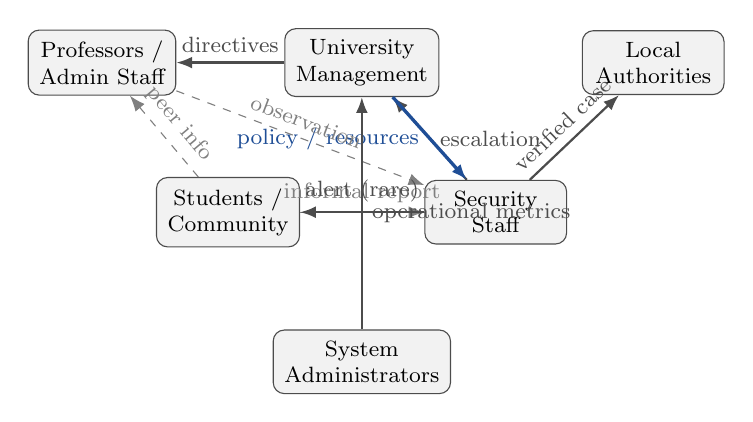
\begin{tikzpicture}[
  font=\footnotesize,
  every node/.style={align=center},
  actor/.style={rounded corners,draw=black!70,fill=soft,
                inner sep=4pt,minimum width=1.8cm,minimum height=0.7cm},
  power/.style={-{Latex[length=2mm]},very thick,loopR},
  info/.style={-{Latex[length=2mm]},thick,black!70},
  weak/.style={-{Latex[length=2mm]},dashed,black!50}
]
\node[actor] (stu)   at (0,0)          {Students /\\Community};
\node[actor] (sec)   at (3.4,0)        {Security\\Staff};
\node[actor] (mgmt)  at (1.7,1.9)      {University\\Management};
\node[actor] (loc)   at (5.4,1.9)      {Local\\Authorities};
\node[actor] (prof)  at (-1.6,1.9)     {Professors /\\Admin Staff};
\node[actor] (adm)   at (1.7,-1.9)     {System\\Administrators};

\draw[weak]  (stu)  -- node[above,sloped]{informal report}  (sec);
\draw[info]  (sec)  -- node[above,sloped]{verified case}    (loc);
\draw[info]  (sec)  -- node[right]{escalation}              (mgmt);
\draw[power] (mgmt) -- node[left]{policy / resources}       (sec);
\draw[weak]  (prof) -- node[above,sloped]{observation}      (sec);
\draw[weak]  (stu)  -- node[above,sloped]{peer info}        (prof);
\draw[info]  (mgmt) -- node[above,sloped]{directives}       (prof);
\draw[info]  (adm)  -- node[right]{operational metrics}     (mgmt);
\draw[info]  (sec)  -- node[above,sloped]{alert (rare)}     (stu);
\end{tikzpicture}
\caption{Stakeholder interaction diagram of the campus safety system.
Solid arrows denote structured, recorded information flows; dashed
arrows denote informal, unrecorded, or low-bandwidth flows; thick
blue arrows denote relations of authority and resource allocation.
The asymmetry is the central finding: information flowing
\emph{into} the security staff is informal and lossy, whereas
information flowing \emph{out of} the security staff toward the
community is structurally underdeveloped. Source: own elaboration (2026).}
\label{fig:stakeholder}
\end{figure}

\subsection{Cause-Effect Analysis of Under-Reporting}
The single most consequential structural deficiency identified in
the data is the gap between actual incidence and recorded incidence.
Fig.~\ref{fig:fishbone} formalizes this in an Ishikawa (fishbone)
diagram, mapping the contributing causes across four conventional
categories.

\begin{figure*}[t]
\centering
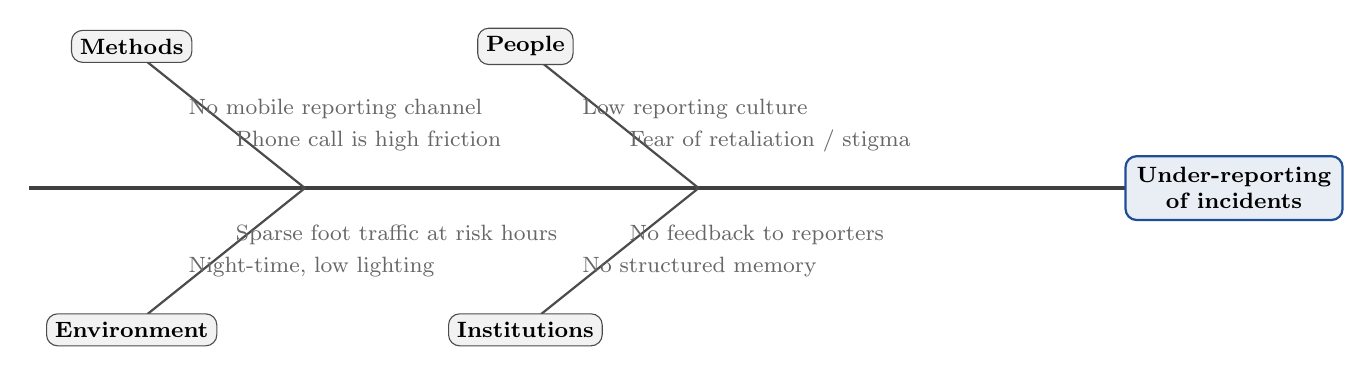
\begin{tikzpicture}[
  font=\footnotesize,
  every node/.style={align=center},
  spine/.style={very thick,->,black!75},
  branch/.style={thick,black!70},
  subbranch/.style={black!60},
  cat/.style={rounded corners,draw=black!70,fill=soft,inner sep=3pt}
]
% Spine
\draw[spine] (-7.5,0) -- (7.0,0);
\node[rounded corners,draw=loopR,thick,fill=loopR!10,inner sep=4pt]
  at (7.8,0) {\textbf{Under-reporting}\\\textbf{of incidents}};

% Upper branches
\draw[branch] (-6,1.6) -- (-4,0);
\node[cat] at (-6.2,1.8) {\textbf{Methods}};
\node at (-5.6,1.0)[anchor=west,subbranch] {No mobile reporting channel};
\node at (-5.0,0.6)[anchor=west,subbranch] {Phone call is high friction};

\draw[branch] (-1,1.6) -- (1,0);
\node[cat] at (-1.2,1.8) {\textbf{People}};
\node at (-0.6,1.0)[anchor=west,subbranch] {Low reporting culture};
\node at (0.0,0.6)[anchor=west,subbranch] {Fear of retaliation / stigma};

% Lower branches
\draw[branch] (-6,-1.6) -- (-4,0);
\node[cat] at (-6.2,-1.8) {\textbf{Environment}};
\node at (-5.6,-1.0)[anchor=west,subbranch] {Night-time, low lighting};
\node at (-5.0,-0.6)[anchor=west,subbranch] {Sparse foot traffic at risk hours};

\draw[branch] (-1,-1.6) -- (1,0);
\node[cat] at (-1.2,-1.8) {\textbf{Institutions}};
\node at (-0.6,-1.0)[anchor=west,subbranch] {No structured memory};
\node at (0.0,-0.6)[anchor=west,subbranch] {No feedback to reporters};
\end{tikzpicture}
\caption{Ishikawa diagram of under-reporting. Each branch maps a class
of root causes contributing to the observed gap between actual and
recorded incidence. The diagram makes explicit that under-reporting
is not attributable to a single failure but to the convergence of
methodological, behavioral, environmental, and institutional factors.
Source: own elaboration (2026).}
\label{fig:fishbone}
\end{figure*}

The diagnostic value of Fig.~\ref{fig:fishbone} is that it constrains
the design space of feasible interventions: any intervention that
addresses only one branch (for example, a purely educational campaign
addressing the People branch) is unlikely to close the under-reporting
gap on its own. This is one of the explicit justifications for
preferring a multi-pronged intervention in
Section~\ref{sec:alternatives}.

\subsection{Information Flow Diagram: Current vs. Target State}
\label{sec:flowdiagram}
Fig.~\ref{fig:flow} presents a side-by-side comparison of the current
information flow (left) and the target information flow under the
proposed intervention (right). The visualization makes the leverage
point explicit: the intervention compresses the chain from event to
response, adds structured memory, and introduces a feedback channel
to the community.

\begin{figure*}[t]
\centering
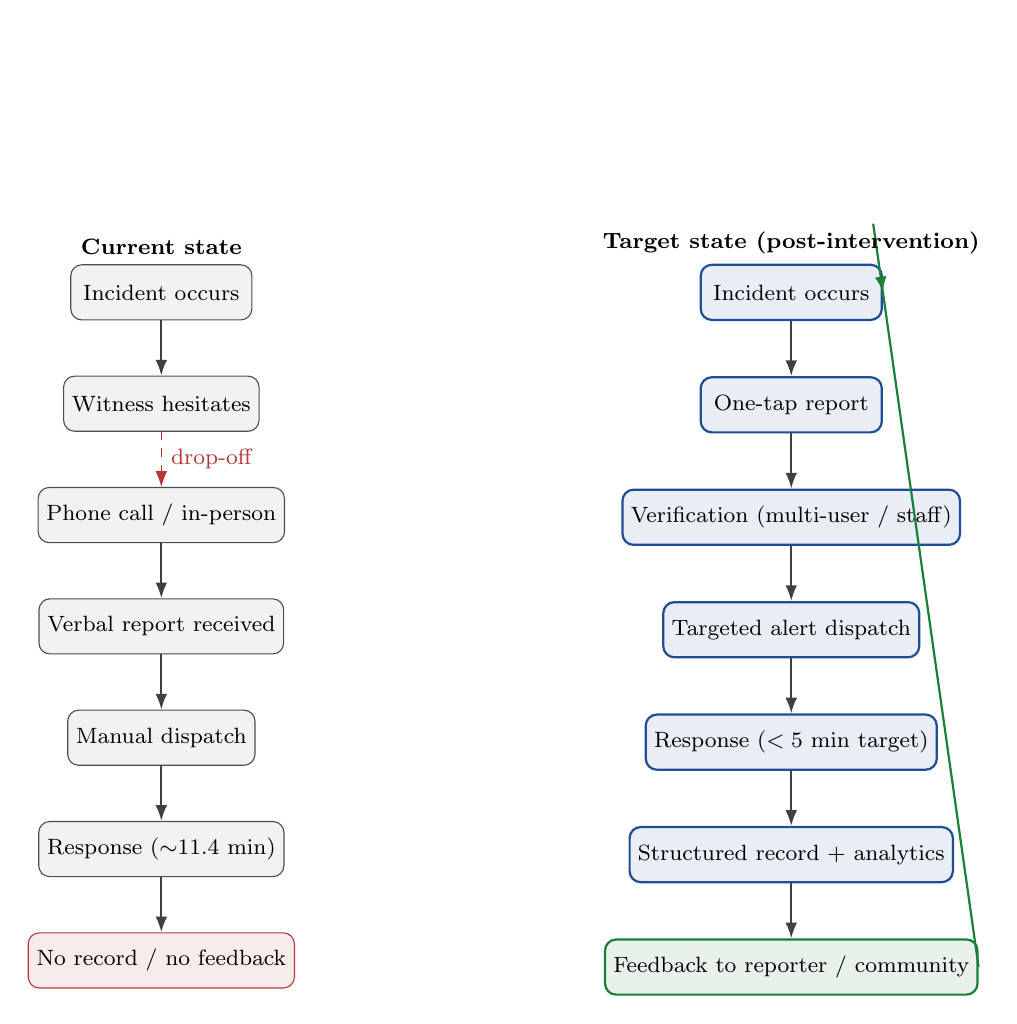
\begin{tikzpicture}[
  font=\footnotesize,
  node distance=0.7cm and 0.7cm,
  every node/.style={align=center},
  flowstep/.style={rounded corners,draw=black!70,fill=soft,
               inner sep=3pt,minimum width=2.3cm,minimum height=0.7cm},
  fast/.style={rounded corners,draw=loopR,thick,fill=loopR!10,
               inner sep=3pt,minimum width=2.3cm,minimum height=0.7cm},
  arr/.style={-{Latex[length=2mm]},thick,black!75},
  loss/.style={-{Latex[length=2mm]},dashed,minus}
]
% LEFT: Current state
\node[flowstep] (e1)  at (-7,3) {Incident occurs};
\node[flowstep] (e2)  [below=of e1]  {Witness hesitates};
\node[flowstep] (e3)  [below=of e2]  {Phone call / in-person};
\node[flowstep] (e4)  [below=of e3]  {Verbal report received};
\node[flowstep] (e5)  [below=of e4]  {Manual dispatch};
\node[flowstep] (e6)  [below=of e5]  {Response (\(\sim\)11.4 min)};
\node[flowstep,fill=minus!10,draw=minus] (e7) [below=of e6] {No record / no feedback};

\draw[arr] (e1) -- (e2);
\draw[loss] (e2) -- (e3) node[midway,right,minus]{drop-off};
\draw[arr] (e3) -- (e4);
\draw[arr] (e4) -- (e5);
\draw[arr] (e5) -- (e6);
\draw[arr] (e6) -- (e7);

\node[anchor=south] at (e1.north) {\textbf{Current state}};

% RIGHT: Target state
\node[fast] (t1) at (1,3) {Incident occurs};
\node[fast] (t2) [below=of t1] {One-tap report};
\node[fast] (t3) [below=of t2] {Verification (multi-user / staff)};
\node[fast] (t4) [below=of t3] {Targeted alert dispatch};
\node[fast] (t5) [below=of t4] {Response (\(<5\) min target)};
\node[fast] (t6) [below=of t5] {Structured record + analytics};
\node[fast,fill=plus!10,draw=plus] (t7) [below=of t6] {Feedback to reporter / community};

\draw[arr] (t1) -- (t2);
\draw[arr] (t2) -- (t3);
\draw[arr] (t3) -- (t4);
\draw[arr] (t4) -- (t5);
\draw[arr] (t5) -- (t6);
\draw[arr] (t6) -- (t7);

% Closing the loop
\draw[arr,plus,bend left=60]
  (t7.east) to[out=0,in=0] (t1.east);

\node[anchor=south] at (t1.north) {\textbf{Target state (post-intervention)}};
\end{tikzpicture}
\caption{Information flow in the campus safety system: current state
(left) and target state under intervention (right). Dashed red arrows
indicate flows with substantial drop-off. The green arrow on the
right closes the feedback loop, transforming the linear current
process into a learning loop. Source: own elaboration (2026).}
\label{fig:flow}
\end{figure*}

%==========================================================================
\section{System Dynamics: Sensitivity, Feedback Loops, and Emergent Behavior}

\subsection{Causal Loop Diagram}
\label{sec:cld}
The static element-relationship view of the previous section is
necessary but insufficient: the campus safety system also exhibits
\emph{dynamic} behavior driven by feedback loops. Fig.~\ref{fig:cld}
presents the causal loop diagram (CLD) of the system. Each arrow is
labeled with a polarity: a positive sign~(+) indicates that the
variables move in the same direction, a negative sign~(\(-\))
indicates that they move in opposite directions. Closed paths form
either reinforcing loops (denoted~\(R\)) or balancing loops
(denoted~\(B\)).

\begin{figure*}[t]
\centering
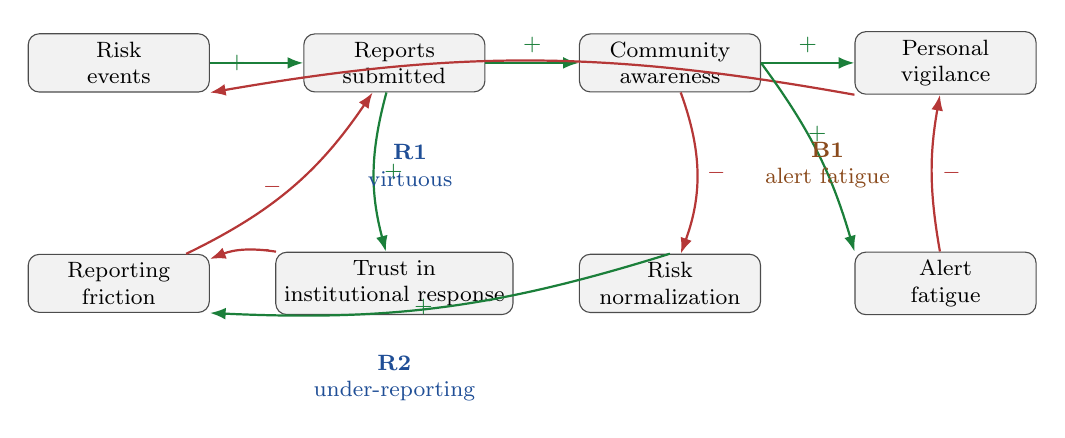
\begin{tikzpicture}[
  font=\footnotesize,
  every node/.style={align=center},
  cldvar/.style={rounded corners,draw=black!70,fill=soft,
              inner sep=3pt,minimum width=2.3cm,minimum height=0.7cm},
  polpos/.style={-{Latex[length=2mm]},thick,plus},
  polneg/.style={-{Latex[length=2mm]},thick,minus},
  ringR/.style={loopR,thick,->},
  ringB/.style={loopB,thick,->}
]
% Variables
\node[cldvar] (incid)  at (-5.5,1.8)  {Risk\\events};
\node[cldvar] (reports)at (-2.0,1.8)  {Reports\\submitted};
\node[cldvar] (aware)  at (1.5,1.8)   {Community\\awareness};
\node[cldvar] (vigil)  at (5.0,1.8)   {Personal\\vigilance};

\node[cldvar] (friction)at (-5.5,-1.0){Reporting\\friction};
\node[cldvar] (trust)   at (-2.0,-1.0){Trust in\\institutional response};
\node[cldvar] (norm)    at (1.5,-1.0) {Risk\\normalization};
\node[cldvar] (fatigue) at (5.0,-1.0) {Alert\\fatigue};

% Arrows: reinforcing loop R1 (virtuous, if active)
\draw[polpos] (reports) -- node[above]{+} (aware);
\draw[polpos] (aware) -- node[above]{+} (vigil);
\draw[polneg] (vigil.south west) to[bend right=10] node[right=2pt]{$-$} (incid.south east);
\draw[polpos] (incid) -- node[left]{+} (reports);

% R2: trust loop
\draw[polpos] (reports) to[bend right=15] node[right]{+} (trust);
\draw[polneg] (trust) to[bend right=15] node[right]{$-$} (friction);
\draw[polneg] (friction) to[bend right=15] node[left]{$-$} (reports);

% Vicious loop: under-reporting -> low awareness -> normalization -> low reporting
\draw[polpos] (norm.north) to[bend left=10] node[left]{+} (friction.south east);
\draw[polneg] (aware) to[bend left=20] node[right]{$-$} (norm);

% Balancing loop B1: alert fatigue
\draw[polpos] (aware.east) to[bend left=10] node[above]{+} (fatigue.north west);
\draw[polneg] (fatigue) to[bend left=10] node[right]{$-$} (vigil);

% Loop labels
\node[loopR] at (-1.8,0.5)  {\textbf{R1}\\virtuous};
\node[loopB] at (3.5,0.5)   {\textbf{B1}\\alert fatigue};
\node[loopR] at (-2.0,-2.2) {\textbf{R2}\\under-reporting};
\end{tikzpicture}
\caption{Causal loop diagram of the campus safety system. Solid green
arrows indicate positive polarity; solid red arrows indicate negative
polarity. Loop R1 is the virtuous reinforcing loop that an effective
intervention seeks to activate; loop R2 is the vicious reinforcing
loop that sustains the current under-reporting state; loop B1 is the
balancing loop that constrains naive amplification of awareness.
Source: own elaboration (2026).}
\label{fig:cld}
\end{figure*}

\subsection{Reinforcing and Balancing Loops}
\label{sec:loops}
Three loops dominate the dynamics of the system, and an effective
intervention must reason about all three simultaneously.

\paragraph{Loop R1 --- Virtuous reinforcement}
Reports submitted increase community awareness, which increases
personal vigilance, which reduces risk events, which reduces the
input to the loop. Inverted, the same loop produces a vicious cycle:
fewer reports lead to lower awareness, which leads to lower vigilance,
which permits more incidents but fewer reports of them. The system
sits today on the vicious side of R1; activating its virtuous mode is
the principal goal of any intervention.

\paragraph{Loop R2 --- Under-reporting trap}
The current state of the system also sustains a self-reinforcing
under-reporting trap: low reporting yields low awareness, which
fosters risk normalization, which increases the perceived friction of
reporting (``why bother if nothing happens?''), which further
suppresses reports. R2 is consistent with the survey finding that
several students who reported having experienced an incident also
reported feeling safe.

\paragraph{Loop B1 --- Alert fatigue}
The balancing counterweight to any awareness-increasing intervention
is alert fatigue: as the volume of alerts grows, the marginal
attention paid to each one falls, and beyond a threshold the
intervention loses signal value. B1 is the system-level reason why
verification matters: without a verification stage, the intervention
amplifies B1 faster than it activates R1, and net effectiveness
declines. The verification component of CSAS is thus not a feature
chosen for engineering elegance but a structural requirement imposed
by the dynamics of the system.

\subsection{Parameter Sensitivity Analysis}
The behavior of the system is dominated by a small set of operational
parameters. Table~\ref{tab:sens} formalizes the analysis by linking
each parameter to its observable effect, the supporting evidence, and
the loop on which it acts.

\begin{table*}[t]
\caption{Parameter Sensitivity Analysis with Loop Attribution}
\label{tab:sens}
\centering
\renewcommand{\arraystretch}{1.2}
\begin{tabular}{p{2.6cm}p{2.5cm}p{4.2cm}p{4.4cm}p{1.8cm}}
\toprule
\textbf{Parameter} & \textbf{Possible change} & \textbf{System effect} & \textbf{Supporting evidence} & \textbf{Acts on} \\
\midrule
Number of reports & Sharp increase & Verification capacity is exceeded, latency rises, B1 dominates & 35\% survey incidence suggests latent volume & R1, B1 \\
User participation & Low engagement & Real risks remain invisible, R2 persists & Low reporting culture across all methods & R1, R2 \\
Time of day & Night-time rise & Incident frequency rises non-linearly & All suspicious events observed in evening/night & R1 \\
Location & High-risk zones & Localized alert clustering & Parking lot consistently identified as highest-risk & R1 \\
Weather conditions & Adverse weather & Visibility drops, movement patterns shift & Both observed suspicious events on rainy nights (hypothesis-grade) & R1 \\
Verification latency & Tighter threshold & Faster alerts at cost of more false positives, accelerating B1 & Trade-off articulated in benchmarking & B1 \\
\bottomrule
\end{tabular}
\end{table*}

\subsection{Non-Linear and Emergent Effects}
Two non-linearities deserve explicit attention. First, the
relationship between active-user count and simultaneous report volume
is non-linear: a small increase in active users can produce a
disproportionately large spike in concurrent reports during
high-activity periods, which stresses the verification stage and may
trigger B1. Second, spatial and temporal clustering means that alert
activity is not uniformly distributed across the campus or the day;
the system therefore requires zone-weighted and time-weighted priority
logic rather than uniform processing of incoming reports. Both
non-linearities are properties of the campus safety system itself,
not of any particular technological artifact, and they constrain the
design of any intervention.

%==========================================================================
\section{Alternative Interventions and Trade-Off Analysis}
\label{sec:alternatives}

\subsection{Candidate Interventions}
Following the system-first principle, the analysis evaluated four
candidate interventions on the campus safety system before settling
on a recommendation:

\begin{enumerate}[leftmargin=*,itemsep=2pt]
\item \textbf{A1 --- Physical-security expansion}: more guards, more
      CCTV coverage, improved lighting in identified risk zones.
\item \textbf{A2 --- Awareness and training programs}: mandatory
      reporting workshops, posters, induction sessions to address
      the reporting-culture branch of Fig.~\ref{fig:fishbone}.
\item \textbf{A3 --- Direct integration with city emergency services}
      (e.g., a 123/911 fast-track from campus).
\item \textbf{A4 --- Crowd-sourced mobile reporting platform with
      verification (CSAS, our proposal)}.
\end{enumerate}

These four alternatives do not exhaust the design space, but they
span the principal dimensions on which interventions can vary
(infrastructure-heavy vs. behavior-focused vs. external-coordination
vs. information-flow-focused).

\subsection{Comparative Evaluation}
Table~\ref{tab:tradeoffs} compares the four candidates on six
criteria derived from the operational gaps quantified in
Section~\ref{sec:gap}.

\begin{table*}[t]
\caption{Trade-Off Comparison of Candidate Interventions}
\label{tab:tradeoffs}
\centering
\renewcommand{\arraystretch}{1.25}
\begin{tabular}{p{3.4cm}cccc}
\toprule
\textbf{Criterion} & \textbf{A1: Physical security} & \textbf{A2: Awareness programs} & \textbf{A3: City emergency integration} & \textbf{A4: CSAS (proposed)} \\
\midrule
Leverage on root cause (info-flow friction) & Low & Medium & Low & High \\
Capital cost & High & Low & Low & Medium \\
Time to deploy & Long (months--years) & Short--medium & Long (procedural) & Short--medium \\
Dependence on external actors & Medium & Low & High & Medium \\
Effect on under-reporting (R2) & Indirect & Direct but slow & None & Direct and structural \\
Risk of triggering B1 (alert fatigue) & Low & Low & Low & Medium (mitigated by verification) \\
\bottomrule
\end{tabular}
\end{table*}

\subsection{Justification of CSAS}
CSAS is recommended because it is the only candidate that acts
directly on the structural variable identified as the system's
binding constraint: the friction of community-to-institution
information flow. A1 raises baseline security but leaves the
under-reporting trap untouched. A2 addresses one branch of the
fishbone but leaves the methods and institutional branches
unchanged; the data do not support the hypothesis that awareness
alone closes the gap. A3 introduces external coordination latency
and does not solve internal reporting. A4---CSAS---combines
mobile-channel design (methods branch), structured memory
(institutional branch), and verification logic (B1 mitigation) in
a single intervention. Crucially, the recommendation is conditional
on the management of the assumptions and unintended consequences
discussed in Section~\ref{sec:risks}; if those assumptions fail,
A4 reduces to A2 plus a software artifact and loses its leverage
advantage.

%==========================================================================
\section{Risks, Assumptions, and Unintended Consequences}
\label{sec:risks}

\subsection{Explicit Assumptions and Validation Status}
The analysis rests on five assumptions whose validation status is
made explicit in Table~\ref{tab:assumptions}. Each row identifies
the assumption, the evidence (if any) currently supporting it, the
classification of its validation status, and the action proposed
to validate it in the next phase.

\begin{table*}[t]
\caption{Explicit Assumptions, Evidence Base, and Validation Plan}
\label{tab:assumptions}
\centering
\renewcommand{\arraystretch}{1.25}
\begin{tabular}{p{0.5cm}p{4.8cm}p{4.2cm}p{1.7cm}p{4.6cm}}
\toprule
\textbf{\#} & \textbf{Assumption} & \textbf{Supporting evidence} & \textbf{Status} & \textbf{Validation action (next phase)} \\
\midrule
A1 & Community members will report if friction is reduced & Survey: 100\% of incident-experienced respondents willing to adopt; benchmarking: high adoption of WhatsApp channels & Plausible & Pilot test with limited cohort, measure actual reporting rate vs. willingness \\
A2 & Verification can be made fast enough for genuine emergencies & Benchmarking: ``slow'' is the principal weakness of existing platforms; design space analysis & Untested & Define explicit latency budget, measure under load \\
A3 & Mobile connectivity is reliable across all campus zones & Not assessed in current observation phase & Unvalidated & Signal-coverage survey across the four observed zones \\
A4 & Verification logic can keep false-positive rate below the B1 threshold & Theoretical: verification narrows the alert stream; no empirical measurement yet & Untested & Define numeric false-positive threshold; simulate or pilot \\
A5 & The campus institutional infrastructure (SIURE, security team) will integrate rather than resist & Interviews: staff articulated a clear need; no formal institutional commitment yet & Partially supported & Stakeholder agreement and integration plan with university administration \\
\bottomrule
\end{tabular}
\end{table*}

\subsection{Risk Register}
Five risks materially affect the intervention. Table~\ref{tab:risks}
characterizes each by likelihood, impact, and proposed mitigation.

\begin{table*}[t]
\caption{Risk Register for the Proposed Intervention}
\label{tab:risks}
\centering
\renewcommand{\arraystretch}{1.25}
\begin{tabular}{p{0.5cm}p{4.4cm}cp{1.6cm}p{1.6cm}p{4.6cm}}
\toprule
\textbf{\#} & \textbf{Risk} & & \textbf{Likelihood} & \textbf{Impact} & \textbf{Mitigation} \\
\midrule
R1 & Low sustained adoption (\(<60\%\) target) & & Medium & High & Institutional endorsement, induction integration \\
R2 & Verification bottleneck under spike loads & & Medium & High & Asynchronous verification queue, staff capacity planning \\
R3 & Connectivity dead-zones break the alert chain & & Medium & Medium & SMS fallback channel; signal-coverage survey \\
R4 & False positives erode trust (B1 dominates) & & Medium & High & Multi-user confirmation, staff moderation, reputation logic \\
R5 & Misuse: harassment reporting weaponized, data privacy breaches & & Low--Medium & High & Reporter anonymity, content moderation, compliance with Ley~1581/2012 \cite{ley1581} \\
\bottomrule
\end{tabular}
\end{table*}

\subsection{Potential Unintended Consequences}
A rigorous systems analysis must anticipate that an intervention
designed to improve a system will also produce effects that are not
part of its design intent. We identify four classes of unintended
consequences:

\paragraph{Vigilantism risk}
A well-functioning awareness channel may encourage community members
to act on reported incidents before institutional responders arrive.
This is undesirable and must be mitigated by the design of the alert
content itself (advisory rather than directive language) and by clear
behavioral guidelines bundled with the platform.

\paragraph{Risk profiling and discrimination}
Aggregated incident data could be used---intentionally or not---to
profile specific zones, demographics, or individuals. The analytics
layer of any implementation must therefore include explicit policies
on aggregation, anonymization, and access control, beyond minimum
compliance with Ley~1581/2012 \cite{ley1581}.

\paragraph{Reduced personal vigilance}
A counterintuitive consequence of an effective alert system is that
community members may delegate vigilance to the platform (``the app
will warn me''), reducing the baseline situational awareness on which
the system itself depends. This is a Goodhart-style risk and is
particularly difficult to detect by quantitative monitoring alone.

\paragraph{Fear amplification}
An accurate alert system makes the system's incident reality visible.
For communities accustomed to low visibility, the initial perception
may be that safety has \emph{worsened}, even though only the
measurement has improved. Management of this perception is a
non-technical implementation requirement.

\subsection{Evaluation Criteria for the Proposed Intervention}
\label{sec:criteria}
The intervention will be evaluated against six criteria mapped to
the operational gaps of Table~\ref{tab:gap}:

\begin{enumerate}[leftmargin=*,itemsep=2pt]
\item \textbf{Median incident-to-response latency} (target: \(< 5\)~min).
\item \textbf{Incident record completeness} (target: \(\geq 85\%\)).
\item \textbf{Sustained community adoption} (target: \(\geq 60\%\) of
      eligible community using the channel at least monthly).
\item \textbf{Alert delivery success rate} (target: \(\geq 99\%\) for
      verified critical alerts).
\item \textbf{False-positive rate on verified alerts} (target: below
      a threshold to be defined empirically based on B1 dynamics).
\item \textbf{Stakeholder satisfaction} (qualitative; campus security
      team, students, and university management surveyed periodically).
\end{enumerate}

These criteria are deliberately stated as observable system-level
metrics, not as features of the artifact.

%==========================================================================
\section{Critical Assessment}
\label{sec:critical}

\subsection{Strengths of the Analysis}
Several elements of this study are methodologically robust. The use
of six complementary data collection methods supports triangulation:
the three structural findings (under-reporting, spatio-temporal
concentration, absence of a centralized channel) appear independently
in interviews, surveys, and direct observation, which provides mutual
validation. All data is primary and collected first-hand, ensuring
traceability. The boundary definition (Section~\ref{sec:boundaries})
is drawn around the phenomenon (campus safety) rather than around the
proposed artifact (CSAS), which keeps the analysis valid independently
of the specific solution adopted. The sensitivity analysis goes beyond
description to identify which parameters dominate system behavior,
which is essential for prioritization in design.

\subsection{Limitations}
The reach of the conclusions is bounded by the limitations summarized
in Table~\ref{tab:limits}. The survey sample of 20 students cannot
support statistical generalization. The observation phase covered
only four zones in eight sessions, leaving indoor spaces and transit
zones uncharacterized. The institutional document analysis was
limited by restricted access to disaggregated data. The
weather-correlation finding is hypothesis-grade only and would require
a longer observation window and more events to support a causal
claim. These limitations define the validation agenda for the next
phase; they do not invalidate the system-level conclusions.

\subsection{Operational Gap Quantification}
\label{sec:gap}
Table~\ref{tab:gap} quantifies the operational gap between the
current state of the campus safety system and the target state that
the intervention seeks to achieve. The gaps are not merely technical;
they reflect deeply embedded behavioral and institutional patterns,
which is why some of them (notably the adoption gap) cannot be closed
by the artifact alone but require parallel institutional action.

\begin{table*}[t]
\caption{Operational Gap Analysis --- Current vs. Target State of the Campus Safety System}
\label{tab:gap}
\centering
\renewcommand{\arraystretch}{1.25}
\begin{tabular}{p{4.5cm}p{4.5cm}p{3.5cm}p{3.5cm}}
\toprule
\textbf{Dimension} & \textbf{Current state} & \textbf{Target state} & \textbf{Gap} \\
\midrule
Incident response time & \(\sim 11.4\)~min (avg.) & \(< 5\)~min & \(-6.4\)~min \\
Community channel adoption & \(\sim 12\%\) & \(\geq 60\%\) & \(-48\)~pp \\
Incident record completeness & \(\sim 41\%\) of events logged & \(\geq 85\%\) & \(-44\)~pp \\
Alert delivery success rate & \(\sim 87\%\) (SMS/call) & \(\geq 99\%\) & \(-12\)~pp \\
\bottomrule
\end{tabular}
\end{table*}

%==========================================================================
\section{Conclusions}

This analysis approached campus safety as a socio-technical system
under study, not as a problem to be solved by a predetermined
technological artifact. Four conclusions follow from that approach,
each formulated as an insight about the system rather than as a
restatement of the proposed solution.

\paragraph{The system is information-bound, not capacity-bound}
The dominant constraint on the campus safety system is the latency
and reliability of the information flow connecting incident,
awareness, and response. This conclusion is supported by the
triangulation of interviews, survey, and observation, and it has a
clear design implication: an intervention that adds enforcement
capacity without addressing the information flow is unlikely to
shift system performance.

\paragraph{The system sits in a self-reinforcing under-reporting trap}
The causal loop analysis shows that the current state of the system
is sustained by a vicious reinforcing loop (R2 in Fig.~\ref{fig:cld}):
low reporting yields low awareness, which fosters risk normalization,
which further suppresses reporting. Breaking this loop requires
acting on the friction of reporting, not on the willingness of
individuals to report---the willingness already exists, as evidenced
by the 100\% adoption intent among incident-experienced respondents.

\paragraph{User participation and verification latency are the dominant parameters}
The sensitivity analysis identifies user participation and
verification latency as the two parameters with the largest
influence on system behavior. The first activates the virtuous loop
R1; the second prevents the balancing loop B1 from dominating. Any
intervention that scores poorly on either parameter cannot succeed,
regardless of its other features.

\paragraph{Verification is not a feature, it is a structural requirement}
The presence of the alert-fatigue balancing loop B1 means that any
intervention that amplifies awareness without filtering necessarily
degrades over time. Verification is therefore not a design preference
but a structural condition for sustainability. This is the most
consequential insight of the analysis for the next phase.

These four insights, together with the assumption-validation plan of
Table~\ref{tab:assumptions} and the unintended-consequence analysis of
Section~\ref{sec:risks}, define the agenda for Workshop No.~2, in
which the system architecture, verification logic, and data model
will be specified as concrete responses to the system-level findings
established here.

%==========================================================================
\begin{thebibliography}{9}

\bibitem{sierra}
C.~A.~Sierra, \emph{TeamWork as Computer Engineers --- CS Collaboration Guidelines}.
Bogot\'a: Universidad Distrital Francisco Jos\'e de Caldas, 2026.

\bibitem{checkland}
P.~Checkland, \emph{Systems Thinking, Systems Practice}.
New York: John Wiley \& Sons, 1981.

\bibitem{meadows}
D.~H.~Meadows, \emph{Thinking in Systems: A Primer}.
White River Junction, VT: Chelsea Green Publishing, 2008.

\bibitem{iso15288}
ISO/IEC/IEEE, \emph{Systems and Software Engineering --- System Life Cycle Processes},
ISO/IEC/IEEE Std.\ 15288:2015, 2015.

\bibitem{creswell}
J.~W.~Creswell and J.~D.~Creswell, \emph{Research Design: Qualitative,
Quantitative, and Mixed Methods Approaches}, 5th ed.
Thousand Oaks, CA: SAGE Publications, 2018.

\bibitem{ley1581}
Congreso de Colombia, \emph{Ley 1581 de 2012 --- R\'egimen General de
Protecci\'on de Datos Personales}, 2012.

\bibitem{senge}
P.~M.~Senge, \emph{The Fifth Discipline: The Art and Practice of the
Learning Organization}. New York: Doubleday, 2006.

\bibitem{sterman}
J.~D.~Sterman, \emph{Business Dynamics: Systems Thinking and Modeling
for a Complex World}. Boston: McGraw-Hill, 2000.

\bibitem{ishikawa}
K.~Ishikawa, \emph{Guide to Quality Control}.
Tokyo: Asian Productivity Organization, 1986.

\end{thebibliography}

\end{document}
